%=====================================================================
%  Trabalho 07 - Reconhecimento de Dígitos com MLP - base MNIST
%  EL056 - Redes Neurais Artificiais - PPGEELT/UFU
%  Compilação: pdflatex -> bibtex -> pdflatex -> pdflatex
%=====================================================================
\documentclass[12pt,a4paper]{article}

%--------------------------- Pacotes ---------------------------------
\usepackage[T1]{fontenc}
\usepackage[utf8]{inputenc}
\usepackage[brazil]{babel}
\usepackage{mathptmx}                 % Times (ABNT)
\usepackage[top=3cm,left=3cm,bottom=2cm,right=2cm]{geometry}
\usepackage{setspace}
\usepackage{indentfirst}
\usepackage{ragged2e}
\usepackage{graphicx}
\usepackage{amsmath,amssymb}
\usepackage{booktabs}
\usepackage{float}
\usepackage[labelsep=endash,font=small,justification=centering,skip=4pt]{caption}
\usepackage{xcolor}
\usepackage{listings}
\usepackage{titlesec}
\usepackage{fancyhdr}
\usepackage[hidelinks]{hyperref}
\usepackage[alf]{abntex2cite}       % citações autor-data (ABNT); após o hyperref

\graphicspath{{figuras/}}

%--------------------- Formatação ABNT -------------------------------
\onehalfspacing
\setlength{\parindent}{1.25cm}
\setlength{\parskip}{0pt}

% Títulos de seção (primária em caixa alta e negrito, secundária em negrito)
\titleformat{\section}{\normalfont\bfseries\MakeUppercase}{\thesection}{0.6em}{}
\titleformat{\subsection}{\normalfont\bfseries}{\thesubsection}{0.6em}{}
\titlespacing*{\section}{0pt}{12pt}{6pt}
\titlespacing*{\subsection}{0pt}{8pt}{4pt}

% Numeração no canto superior direito
\pagestyle{empty}
\fancypagestyle{abnt}{%
  \fancyhf{}\fancyhead[R]{\small\thepage}%
  \renewcommand{\headrulewidth}{0pt}}
\setlength{\headheight}{15pt}

% Fonte das figuras e tabelas (abaixo do elemento, ABNT)
\newcommand{\fonte}[1]{\par\vspace{2pt}{\small Fonte: #1}\par}

% Legenda acima do elemento para figuras e tabelas
\captionsetup[figure]{position=top}
\captionsetup[table]{position=top}

%--------------------- Listagens (Apêndice A) ------------------------
\definecolor{fundocod}{HTML}{F7F7F5}
\definecolor{comentario}{HTML}{52514E}
\definecolor{palavra}{HTML}{1C5CAB}
\definecolor{cadeia}{HTML}{A8481C}
\lstset{
  language=Python,
  basicstyle=\ttfamily\scriptsize,
  keywordstyle=\color{palavra}\bfseries,
  commentstyle=\color{comentario}\itshape,
  stringstyle=\color{cadeia},
  backgroundcolor=\color{fundocod},
  numbers=left, numberstyle=\tiny\color{comentario}, numbersep=6pt,
  frame=single, rulecolor=\color{gray!40},
  breaklines=true, breakatwhitespace=false,
  postbreak=\mbox{\textcolor{comentario}{$\hookrightarrow$}\space},
  showstringspaces=false, tabsize=4, columns=fullflexible, keepspaces=true,
  extendedchars=true, inputencoding=utf8,
  literate=
    {á}{{\'a}}1 {à}{{\`a}}1 {â}{{\^a}}1 {ã}{{\~a}}1
    {é}{{\'e}}1 {ê}{{\^e}}1 {í}{{\'i}}1
    {ó}{{\'o}}1 {ô}{{\^o}}1 {õ}{{\~o}}1 {ú}{{\'u}}1 {ü}{{\"u}}1
    {ç}{{\c{c}}}1
    {Á}{{\'A}}1 {À}{{\`A}}1 {Â}{{\^A}}1 {Ã}{{\~A}}1
    {É}{{\'E}}1 {Ê}{{\^E}}1 {Í}{{\'I}}1
    {Ó}{{\'O}}1 {Ô}{{\^O}}1 {Õ}{{\~O}}1 {Ú}{{\'U}}1
    {Ç}{{\c{C}}}1 {º}{{\textordmasculine}}1 {ª}{{\textordfeminine}}1
}

%--------------------- Capa e folha de rosto -------------------------
%=====================================================================
%  BLOCO REUTILIZAVEL: CAPA + FOLHA DE ROSTO (ABNT NBR 14724)
%  Extraido do modelo fornecido pelo usuario (PPGEELT/UFU).
%  Este arquivo e' pensado para ser colado no preambulo (antes de
%  \begin{document}) de qualquer trabalho que precise da mesma capa.
%=====================================================================

%--------------------------- Logos opcionais --------------------------
\newcommand{\logoou}[2]{%
  \IfFileExists{#1}{\includegraphics[height=#2,width=\linewidth,keepaspectratio]{#1}}%
                   {\rule{0pt}{#2}}}

%=====================================================================
%  >>>>>>>>>>>>>>  PREENCHA AQUI OS DADOS DO TRABALHO  <<<<<<<<<<<<<<
%=====================================================================
\newcommand{\vazio}{}   % marcador interno para campos opcionais -- nao altere

% AJUSTE AQUI conforme necessario:
\newcommand{\Autor}{LUCAS ALBINO MARTINS\\12622EEL006}
\newcommand{\Titulo}{Trabalho 07 -- Reconhecimento de D\'igitos com Perceptron Multicamadas na Base MNIST}
\newcommand{\Subtitulo}{Disciplina: EL056 - Redes Neurais Artificiais}
\newcommand{\Orientador}{Prof. Dr. Keiji Yamanaka}
\newcommand{\Coorientador}{}                    % vazio se nao houver
\newcommand{\Matricula}{}                       % vazio para omitir
\newcommand{\Local}{Uberl\^andia}
\newcommand{\Ano}{2026}

% ---- Titulo do elemento textual (cabecalho da 1a pagina de texto) ----
\newcommand{\TituloTexto}{Reconhecimento de d\'igitos manuscritos do MNIST
com Perceptron Multicamadas treinado por backpropagation}

% ---- Nota de apresentacao da folha de rosto --------------------------
\newcommand{\NotaApresentacao}{%
  Trabalho apresentado ao Programa de P\'os-Gradua\c{c}\~ao em Engenharia
  El\'etrica (PPGEELT) da Universidade Federal de Uberl\^andia como
  requisito parcial de avalia\c{c}\~ao da disciplina.

  \vspace{0.45cm}
  Disciplina: EL056 - Redes Neurais Artificiais.

  \vspace{0.45cm}
  Professor: \Orientador.
  \ifx\Coorientador\vazio\else

    \vspace{0.2cm}
    Coorientador: \Coorientador.
  \fi
}

%--------------------- Logos (pasta logos/) ------------------------------------------
\newcommand{\LogoEsquerda}{logos/logo-ppgeel.png}
\newcommand{\LogoDireita}{logos/logo-ufu.png}
\newcommand{\AlturaLogoEsq}{2.2cm}   % ajuste fino da altura de cada logo
\newcommand{\AlturaLogoDir}{2.6cm}

%=====================================================================
%  CABECALHO INSTITUCIONAL (logos + nome da instituicao + filete)
%=====================================================================
\newcommand{\cabecalhoinstitucional}{%
  \begin{center}
    \noindent
    \begin{minipage}[c]{0.19\textwidth}
      \raggedright
      \logoou{\LogoEsquerda}{\AlturaLogoEsq}
    \end{minipage}%
    \hfill
    \begin{minipage}[c]{0.58\textwidth}
      \centering
      \singlespacing
      {\fontsize{12}{15}\selectfont\bfseries
        UNIVERSIDADE FEDERAL DE UBERL\^ANDIA\par}
      \vspace{0.25cm}
      {\fontsize{12}{15}\selectfont
        PPGEELT -- P\'os-Gradua\c{c}\~ao em Engenharia El\'etrica\par}
    \end{minipage}%
    \hfill
    \begin{minipage}[c]{0.19\textwidth}
      \raggedleft
      \logoou{\LogoDireita}{\AlturaLogoDir}
    \end{minipage}

    \vspace{0.35cm}
    \rule{\textwidth}{1.1pt}
  \end{center}
}

%=====================================================================
%  CAPA -- ABNT NBR 14724
%=====================================================================
\newcommand{\fazcapa}{%
  \thispagestyle{empty}
  \begin{center}
    \cabecalhoinstitucional

    \vspace{2.5cm}

    {\fontsize{12}{15}\selectfont\MakeUppercase{\Autor}\par}

    \ifx\Matricula\vazio\else
      \vspace{0.4cm}
      {\fontsize{11}{14}\selectfont Matr\'icula: \Matricula\par}
    \fi

    \vspace{4.0cm}

    {\fontsize{16}{20}\selectfont\bfseries\MakeUppercase{\Titulo}\par}
    \ifx\Subtitulo\vazio\else
      \vspace{0.35cm}
      {\fontsize{13}{16}\selectfont\Subtitulo\par}
    \fi

    \vfill

    {\fontsize{12}{15}\selectfont \Local\par}
    \vspace{0.15cm}
    {\fontsize{12}{15}\selectfont \Ano\par}
  \end{center}
  \newpage
  \setcounter{page}{1}   % a contagem ABNT comeca na folha de rosto
}

%=====================================================================
%  FOLHA DE ROSTO -- ABNT NBR 14724
%=====================================================================
\newcommand{\fazfolhaderosto}{%
  \thispagestyle{empty}
  \begin{center}
    \cabecalhoinstitucional

    \vspace{2.0cm}

    {\fontsize{12}{15}\selectfont\MakeUppercase{\Autor}\par}

    \vspace{3.0cm}

    {\fontsize{16}{20}\selectfont\bfseries\MakeUppercase{\Titulo}\par}
    \ifx\Subtitulo\vazio\else
      \vspace{0.35cm}
      {\fontsize{13}{16}\selectfont\Subtitulo\par}
    \fi
  \end{center}

  \vspace{2.0cm}

  \hfill
  \begin{minipage}{0.5\textwidth}
    \singlespacing
    \setlength{\parindent}{0pt}
    \fontsize{10}{12}\selectfont
    \justifying
    \NotaApresentacao
  \end{minipage}

  \vfill

  \begin{center}
    {\fontsize{12}{15}\selectfont \Local\par}
    \vspace{0.15cm}
    {\fontsize{12}{15}\selectfont \Ano\par}
  \end{center}
  \newpage
}


\begin{document}

\fazcapa
\fazfolhaderosto

%============================ RESUMO =================================
\thispagestyle{empty}
\begin{center}\textbf{RESUMO}\end{center}
\vspace{2pt}
\begin{singlespace}
\noindent
Este trabalho apresenta o treinamento de um Perceptron Multicamadas (MLP) para o
reconhecimento dos dígitos manuscritos da base MNIST, com 60.000 imagens de treino e 10.000
de teste em $28\times28$ pixels, convertidas para a representação bipolar. A rede tem uma
camada oculta de 100 neurônios com ativação tangente hiperbólica e foi implementada do
zero em NumPy, com treinamento por \textit{backpropagation} com momento em mini-lotes. O
critério de parada foi atingido em 26 épocas, e a rede obteve 96,93\% de acurácia no
conjunto de teste. Com 10\% dos pixels invertidos, a acurácia média foi de 91,76\%, e com
20\%, de 76,44\%. Sem o termo de momento, a tolerância não foi atingida em 30 épocas. A rede
treinada apenas com dígitos manuscritos reconheceu 90\% dos dígitos impressos nas cinco
fontes do enunciado. No estudo de sensibilidade, a acurácia de teste subiu de 93,43\% com
25 neurônios ocultos para 97,21\% com 200.

\vspace{6pt}
\noindent\textbf{Palavras-chave:} redes neurais artificiais; perceptron multicamadas;
\textit{backpropagation}; MNIST; reconhecimento de dígitos.
\end{singlespace}
\newpage

%============================ SUMÁRIO ================================
\thispagestyle{empty}
\renewcommand{\contentsname}{\centering SUMÁRIO}
\begin{singlespace}
\tableofcontents
\end{singlespace}
\newpage

%============================ TEXTO ==================================
\pagestyle{abnt}

\section{Introdução}

O reconhecimento de dígitos manuscritos é um problema clássico de classificação de
padrões. A base MNIST, apresentada por \citeonline{lecun1998}, tornou-se a referência para
comparar classificadores nessa tarefa: ela reúne 70.000 dígitos escritos por centenas de
pessoas, normalizados e centralizados em imagens de $28\times28$ pixels. O mesmo trabalho
mostra que um perceptron multicamadas com uma camada oculta, treinado por
\textit{backpropagation} \cite{rumelhart1986}, já alcança taxas de erro de poucos por cento.

O enunciado pede o treinamento de uma MLP para reconhecer dígitos. Nesta versão, a base de
treinamento é o MNIST, e os dígitos impressos nas cinco fontes do enunciado entram como
teste adicional, com dígitos que a rede não viu no treinamento. Os objetivos são
implementar a MLP e o algoritmo de treinamento sem bibliotecas de redes neurais e avaliar
a acurácia, a robustez a ruído, o efeito do momento, o efeito do número de neurônios
ocultos e a generalização para dígitos impressos.

\section{Fundamentação teórica}

\subsection{Perceptron multicamadas}

A MLP é uma rede alimentada adiante em que uma ou mais camadas de neurônios ocultos, com
ativação não linear, permitem aprender fronteiras de decisão não lineares
\cite{haykin2009,braga2007}. Com $n$ entradas $x_i$, $p$ neurônios ocultos $z_j$ e $m$
saídas $y_k$, e usando a notação de \citeonline{fausett1994}, a fase direta é
\begin{equation}
z_j = f\Big(v_{0j} + \sum_{i=1}^{n} x_i v_{ij}\Big), \qquad
y_k = f\Big(w_{0k} + \sum_{j=1}^{p} z_j w_{jk}\Big),
\end{equation}
em que $v_{0j}$ e $w_{0k}$ são os bias e $f(x)=\tanh(x)$, com $f'(x)=1-f(x)^2$.

\subsection{Backpropagation em mini-lotes}

O treinamento minimiza o erro quadrático $E=\frac12\sum_k (t_k-y_k)^2$ por descida de
gradiente. A regra delta generalizada \cite{rumelhart1986} calcula os termos de erro
\begin{equation}
\delta_k = (t_k-y_k)\,f'(y\_in_k), \qquad
\delta_j = f'(z\_in_j)\sum_{k=1}^{m}\delta_k\,w_{jk}.
\end{equation}
No algoritmo padrão a padrão, os pesos são corrigidos após cada exemplo. Com dezenas de
milhares de exemplos, é usual corrigir os pesos com a média dos gradientes de um pequeno
lote de $B$ padrões \cite{haykin2009}, o que reduz o custo computacional e o ruído das
atualizações.

\subsection{Termo de momento}

Cada correção recebe uma fração $\mu$ da correção anterior \cite{fausett1994,haykin2009}:
\begin{equation}
\Delta w_{jk}(t) = \frac{\alpha}{B}\sum_{p\,\in\,\text{lote}}\delta_k^{(p)} z_j^{(p)}
+ \mu\,\Delta w_{jk}(t-1),
\end{equation}
e analogamente para $v_{ij}$, com $z_0=x_0=1$ para os bias. Com $B=1$ e $\mu=0$ obtém-se o
algoritmo padrão a padrão sem momento.

\section{Metodologia}

\subsection{Base de dados e pré-processamento}

Os quatro arquivos originais do MNIST (formato IDX) foram lidos diretamente com NumPy
\cite{harris2020}. As intensidades (0 a 255) foram normalizadas para $[0,1]$ e binarizadas
em 0,5: tinta vale $+1$ e fundo, $-1$. Cada padrão tem 784 entradas, das quais, em média,
103,7 são de tinta. As 5.000 últimas imagens do treino formam o conjunto de validação,
usado para escolher a melhor época; restam 55.000 para treino. O conjunto de teste (10.000
imagens) foi usado apenas na avaliação final. A Figura~\ref{fig:base} mostra exemplos.

\begin{figure}[H]
  \centering
  \caption{Cinco exemplos de cada dígito do conjunto de teste, binarizados (preto $=+1$)}
  \label{fig:base}
  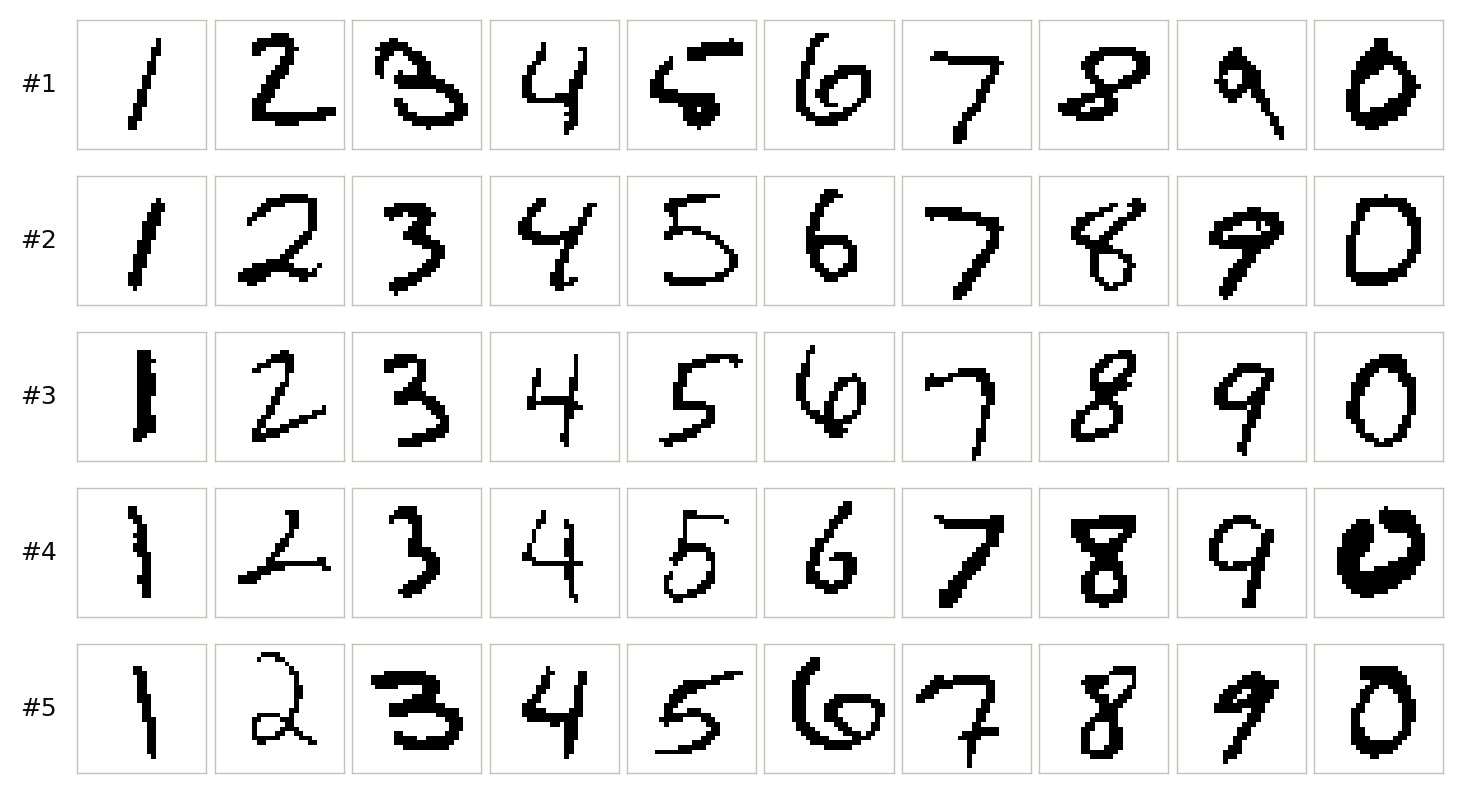
\includegraphics[width=0.62\textwidth]{fig_base_dados.png}
  \fonte{elaborada pelo autor (2026) a partir da base MNIST.}
\end{figure}

Para o teste com dígitos impressos, os dez dígitos de cada uma das cinco fontes do
enunciado (F1 -- DejaVu Sans Bold; F2 -- Liberation Serif; F3 -- DejaVu Sans ExtraLight;
F4 -- Kalam, manuscrita; F5 -- DejaVu Serif Condensed) passaram pelo pré-processamento do
MNIST \cite{lecun1998}: ajuste a uma caixa de $20\times20$ pixels com a proporção mantida,
centralização pelo centro de massa numa imagem de $28\times28$ e a mesma binarização
(Figura~\ref{fig:fontes}).

\subsection{Arquitetura e hiperparâmetros}

A rede tem 784 entradas, 100 neurônios ocultos e 10 saídas com codificação bipolar
\textit{one-hot}; a classe atribuída é a do neurônio de maior saída. O treinamento para
quando o erro quadrático médio por padrão, $E_{\text{total}}/P$, fica abaixo da tolerância
ou no limite de épocas, e ao final restauram-se os pesos da época de maior acurácia de
validação (Tabela~\ref{tab:hiper}).

\begin{table}[H]
  \centering
  \caption{Hiperparâmetros da MLP}
  \label{tab:hiper}
  \begin{tabular}{lc}
    \toprule
    Parâmetro & Valor \\
    \midrule
    Arquitetura & 784--100--10 \\
    Taxa de aprendizagem $\alpha$ & 0,01 \\
    Momento $\mu$ & 0,5 \\
    Tamanho do lote $B$ & 32 \\
    Tolerância de $E_{\text{total}}/P$ & 0,05 \\
    Máximo de épocas & 30 \\
    Pesos iniciais & $U(-1/\sqrt{n};\,1/\sqrt{n})$, semente 2026 \\
    \bottomrule
  \end{tabular}
  \fonte{elaborada pelo autor (2026).}
\end{table}

Na inicialização, $n$ é o número de entradas do neurônio, incluindo o bias. Com 784
entradas, uma amplitude fixa como $\pm0{,}5$ satura a $\tanh$ desde o início. Em ensaios
preliminares, $\alpha=0{,}05$ com $\mu=0{,}9$ fez o treinamento divergir, o que levou aos
valores da Tabela~\ref{tab:hiper}.

Os experimentos foram: (i) o treinamento principal e o mesmo treinamento sem momento;
(ii) acurácia e matriz de confusão no teste; (iii) robustez a ruído, invertendo 5, 10, 15
e 20\% dos pixels de cada imagem de teste em 30 repetições por nível; (iv) teste com os 50
dígitos impressos; (v) sensibilidade a 25, 50, 100 e 200 neurônios ocultos, com até 20
épocas cada.

\section{Resultados}

\subsection{Treinamento}

O erro quadrático médio por padrão caiu de 0,3041 na primeira época para 0,0500 na época
26, quando a tolerância foi atingida, após 36,8~s de treinamento. A maior acurácia de
validação, 97,74\%, ocorreu na época 23, cujos pesos foram mantidos. Sem momento, o erro
estava em 0,1407 na época 10 e em 0,0936 na época 20, contra 0,1061 e 0,0640 com momento, e
terminou as 30 épocas em 0,0694, sem atingir a tolerância (Figura~\ref{fig:erro}). Na
validação, o melhor resultado sem momento foi de 97,52\%.

\begin{figure}[H]
  \centering
  \caption{Erro quadrático médio por padrão e acurácia de validação por época}
  \label{fig:erro}
  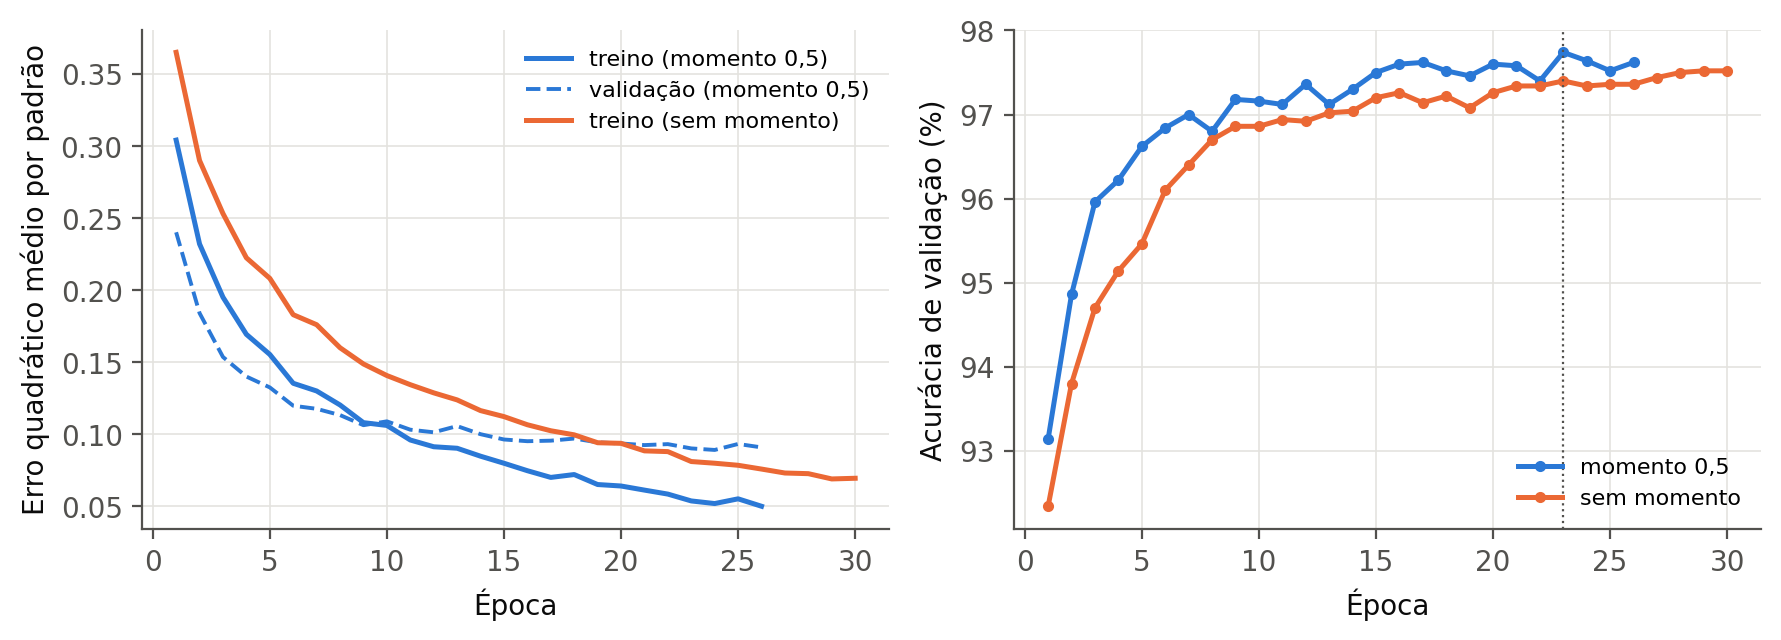
\includegraphics[width=0.95\textwidth]{fig_curva_erro.png}
  \fonte{elaborada pelo autor (2026).}
\end{figure}

\subsection{Acurácia no teste e matriz de confusão}

A acurácia foi de 98,70\% no treino e de 96,93\% no teste (307 erros em 10.000); a rede sem
momento obteve 96,89\% no teste. Por classe, a acurácia variou de 95,33\% (dígito 7) a
98,94\% (dígito 1). As confusões mais frequentes foram 7 $\to$ 1 (14 casos), 7 $\to$ 2 (12),
4 $\to$ 9 (12), 9 $\to$ 4 (11) e 3 $\to$ 5 (11) (Figura~\ref{fig:confusao}).

\begin{figure}[H]
  \centering
  \caption{Matriz de confusão no conjunto de teste (cores em escala logarítmica)}
  \label{fig:confusao}
  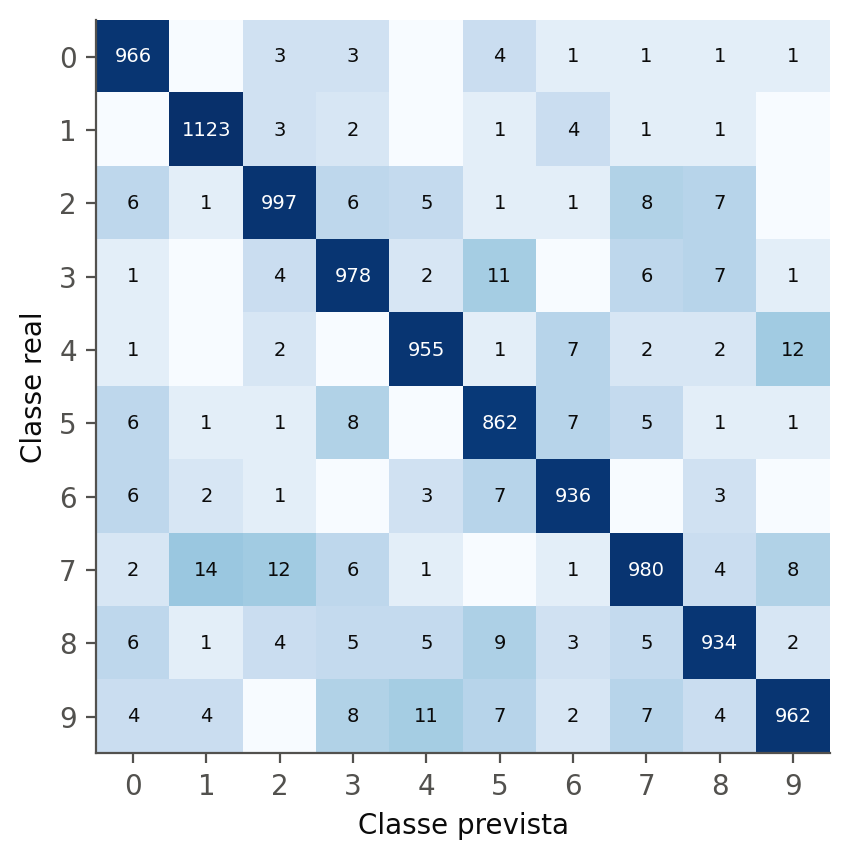
\includegraphics[width=0.55\textwidth]{fig_confusao.png}
  \fonte{elaborada pelo autor (2026).}
\end{figure}

\subsection{Robustez a ruído}

A acurácia média caiu para 95,28\% com 5\% dos pixels invertidos, 91,76\% com 10\%, 85,56\%
com 15\% e 76,44\% com 20\%, com desvios padrão inferiores a 0,4 ponto percentual entre as
30 repetições (Figura~\ref{fig:ruido}).

\begin{figure}[H]
  \centering
  \caption{Acurácia média no teste em função do nível de ruído (30 repetições)}
  \label{fig:ruido}
  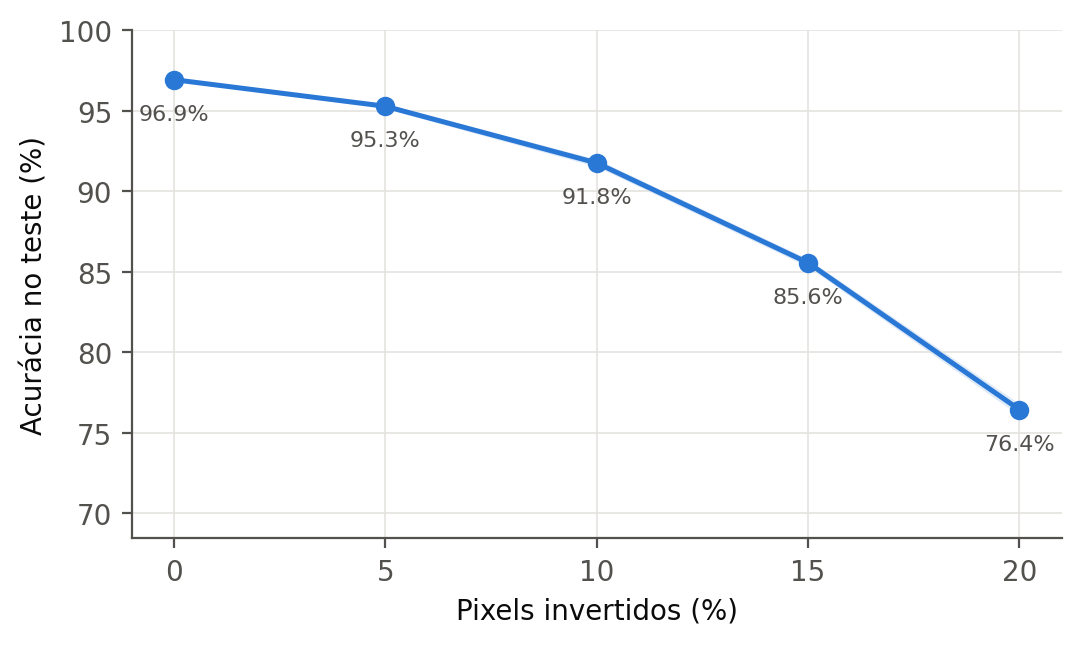
\includegraphics[width=0.62\textwidth]{fig_ruido.png}
  \fonte{elaborada pelo autor (2026).}
\end{figure}

\subsection{Dígitos impressos}

A rede reconheceu 45 dos 50 dígitos impressos (90\%). As fontes F4 (manuscrita) e F5
(serifada condensada) tiveram 100\%, F1 teve 90\% (erro 1 $\to$ 2) e F2 e F3 tiveram 80\%
(erros 4 $\to$ 5 e 8 $\to$ 0 em F2; 4 $\to$ 5 e 9 $\to$ 8 em F3).

\begin{figure}[H]
  \centering
  \caption{Dígitos das cinco fontes no formato do MNIST (F1 a F5, de cima para baixo)}
  \label{fig:fontes}
  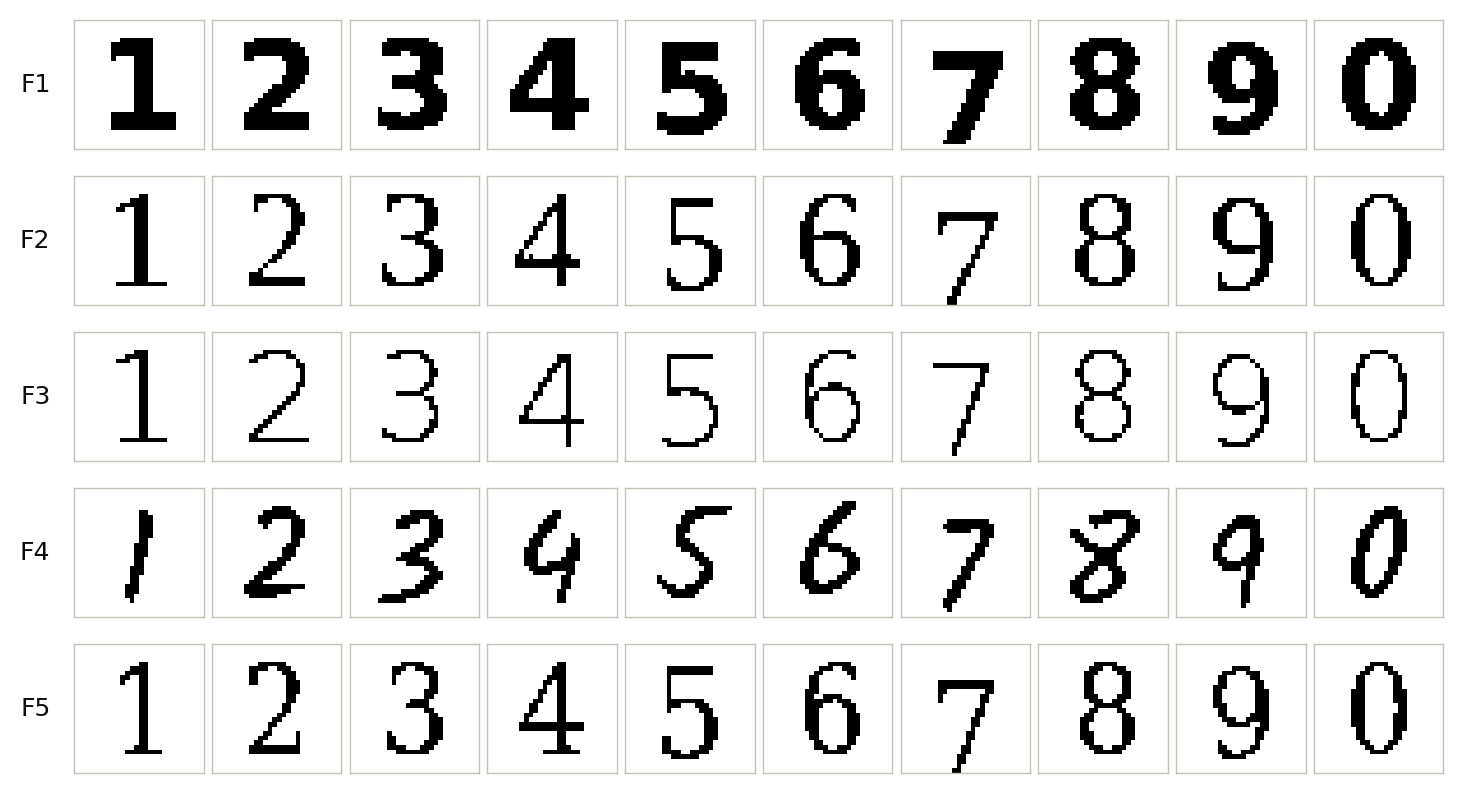
\includegraphics[width=0.62\textwidth]{fig_fontes_mnist.png}
  \fonte{elaborada pelo autor (2026).}
\end{figure}

\subsection{Sensibilidade ao número de neurônios ocultos}

A Tabela~\ref{tab:sens} mostra que a acurácia cresce com o número de neurônios ocultos, com
ganhos cada vez menores, enquanto o número de pesos e o tempo de treinamento crescem
aproximadamente na mesma proporção. Com 100 neurônios, o resultado (96,83\%) difere do
treinamento principal (96,93\%) porque o estudo limita o treino a 20 épocas.

\begin{table}[H]
  \centering
  \caption{Efeito do número de neurônios ocultos (até 20 épocas)}
  \label{tab:sens}
  \begin{tabular}{ccccc}
    \toprule
    Ocultos & Pesos & Teste (\%) & Teste com 10\% de ruído (\%) & Tempo (s) \\
    \midrule
    25  & 19.885  & 93,43 & 85,91 & 7,9 \\
    50  & 39.760  & 95,77 & 88,81 & 14,5 \\
    100 & 79.510  & 96,83 & 91,92 & 27,8 \\
    200 & 159.010 & 97,21 & 92,70 & 46,8 \\
    \bottomrule
  \end{tabular}
  \fonte{elaborada pelo autor (2026).}
\end{table}

\section{Discussão}

A acurácia de 96,93\% está no patamar esperado para uma MLP de uma camada oculta no MNIST
\cite{lecun1998}, mesmo com as entradas binarizadas, que descartam os tons de cinza das
bordas. Os erros se concentram em pares de traçado semelhante: um 7 sem a barra superior
longa se parece com um 1; o 4 fechado se confunde com o 9; o 3 e o 5 diferem apenas na
metade superior.

O momento acelerou a redução do erro de treinamento: com $\mu=0{,}5$, a tolerância foi
atingida em 26 épocas, o que não aconteceu em 30 épocas sem momento. A diferença de
acurácia no teste, porém, foi pequena (96,93\% contra 96,89\%). Na prática, o momento
encurta o treinamento sem mudar a qualidade final da solução.

Com 784 pixels, a robustez a ruído é menor que a observada com os 50 padrões em grade
$12\times9$ do trabalho anterior: aqui a rede precisa separar milhares de variações de
escrita, e as fronteiras entre as classes ficam mais próximas dos exemplos. Inverter 20\%
dos pixels (157 de 784) cria, em média, cerca de 136 pontos de tinta no fundo, mais do que
a tinta de um dígito típico (103,7 pixels), e mesmo assim a rede acerta três de cada quatro
imagens.

O teste com dígitos impressos inverte o resultado do trabalho com fontes: lá a fonte
manuscrita era a mais difícil, e aqui foi reconhecida integralmente, por se parecer com os
dados de treino. Os erros apareceram nas fontes de traço uniforme e com serifas, como o 4
fechado de F2 e F3 confundido com 5. A sensibilidade mostra que 25 neurônios já fornecem
uma solução razoável e que dobrar a camada oculta a partir de 100 neurônios traz pouco
ganho (0,38 ponto percentual) pelo dobro de pesos.

\section{Conclusão}

A MLP implementada do zero e treinada no MNIST alcançou 96,93\% de acurácia no teste, com
degradação gradual sob ruído (91,76\% com 10\% dos pixels invertidos). O momento reduziu o
tempo até a convergência, e o número de neurônios ocultos mostrou retornos decrescentes a
partir de 100. A rede, treinada apenas com dígitos manuscritos, reconheceu 90\% dos dígitos
impressos nas cinco fontes do enunciado. Como continuidade, seria possível usar as
intensidades em tons de cinza, ampliar a base com pequenas deformações dos dígitos ou
acrescentar dígitos impressos ao treino.

%========================== REFERÊNCIAS ==============================
\newpage
\pagestyle{abnt}
\begin{singlespace}
\bibliography{referencias}
\end{singlespace}

%=========================== APÊNDICE ================================
\newpage
\section*{APÊNDICE A -- CÓDIGO-FONTE EM PYTHON}
\addcontentsline{toc}{section}{APÊNDICE A -- CÓDIGO-FONTE EM PYTHON}
\noindent Arquivo \texttt{trabalho07\_mnist.py}, executado com
\texttt{python trabalho07\_mnist.py}.
\begin{singlespace}
\lstinputlisting{trabalho07_mnist.py}
\end{singlespace}

\end{document}
